\subsection*{Questions 1 through 4}

\colorbox{BurntOrange!25}{ \parbox{\textwidth}{
    \textbf{\textit{\underline{Question}}}:
\textit{\begin{enumerate}
    \item Label and interpret the model ingredients properly.
    \item Characterise the individual labor supply curve.
    \item Characterise the aggregate labor supply curve.
    \item Characterise the aggregate labor demand curve
\end{enumerate}}}}\\

\colorbox{BurntOrange!25}{\textbf{\textit{\underline{Step 1A}}}: Working households $\to$ intensive margin labour supply.}
Start with the working household's problem.
\begin{equation}
    \begin{aligned}
    &W(a, z)  = \max _{c, n, a^{\prime}} \left\{ \log (c)-\eta \frac{1}{1+\frac{1}{\chi}} n^{1+\frac{1}{\chi}}+\beta v\left(a^{\prime}\right)\right\} \\
    &\text {s.t.} \;  c+a^{\prime}=z w(1-\tau) n+a(1+r(1-\tau))+T
\end{aligned}
\end{equation}
Construct the Lagrangian, assuming that $v\left(a^{\prime}\right)=\log\left(a^{\prime}\right)$:
\begin{equation}
    \mathcal{L}=\log (c)-\eta \frac{1}{1+\frac{1}{\chi}} n^{1+\frac{1}{\chi}}+\beta \log \left(a^{\prime}\right)+\lambda \left[z w(1-\tau) n+a(1+r(1-\tau))+T-c-a^{\prime} \right].
\end{equation}
The first-order conditions are as follows:
\begin{subequations}
    \begin{align}
        & \mathcal{L}_c= \frac{1}{c}+\lambda=0 \implies \lambda = \frac{1}{c}, \\
        & \mathcal{L}_n = -\eta n^{\frac{1}{\chi}}+\lambda zw (1-\tau)=0 \implies \eta n^{\frac{1}{\chi}}=\frac{zw (1-\tau)}{c}, \label{a1_foc1}
    \end{align}
    and 
    \begin{align}
        \mathcal{L}_{a^\prime}=\frac{\beta}{a^\prime}-\lambda =0 \implies a^\prime = \beta c.\label{a1_foc2}
    \end{align}
\end{subequations}
Combine the results of Equations \eqref{a1_foc1} and \eqref{a1_foc2} with the budget contraint to arrive at the Euler equation:
\begin{subequations}
    \begin{align}
        &  \underbrace{ \textcolor{BurntOrange}{c+a^{\prime}}}_{\text{Use \eqref{a1_foc2}}}=\underbrace{z w(1-\tau) \textcolor{BurntOrange}{n}}_{\text{Use \eqref{a1_foc1}}}+a(1+r(1-\tau))+T, \\
        &  \boxed{c(1+\beta)=z w(1-\tau) \left( \frac{z w(1-\tau)}{\eta c}\right)^\chi +a(1+r(1-\tau))+T.} \tag{WH-ILS}\label{a1_euler} 
    \end{align}
\end{subequations}
Equation \eqref{a1_euler} governs the \textcolor{BurntOrange}{\textbf{intensive labour supply of a working household}},  
 $c_w^\star (a,z)$ is their consumption level.\\ 

 Further, notice that $c_w^\star (a,z)$ increases in $z$:
 \begin{subequations}
    \begin{align}
        & \frac{\partial c_w^\star (a,z)}{\partial z} (1+\beta)=\underbrace{\left[w (1-\tau) \eta^{-1} \right]^{1+\chi}}_{\equiv \theta >0 }\times  \frac{(1+\chi)z^\chi c_w^\star (a,z) - z^\chi \frac{\partial c_w^\star (a,z)}{\partial z} }{c_w^\star (a,z)^2} \implies \\
        & \frac{\partial c_w^\star (a,z)}{\partial z} \left(1+\beta +\theta \frac{z^\chi}{c_w^\star (a,z)^2}\right)= \frac{\theta  (1+\chi) z^\chi }{c_w^\star (a,z)} \implies \\
        & \frac{\partial c_w^\star (a,z)}{\partial z} = \frac{\frac{\theta  (1+\chi) z^\chi }{c_w^\star (a,z)} }{1+\beta +\theta \frac{z^\chi}{c_w^\star (a,z)^2}} >0. 
    \end{align}
 \end{subequations}
Also, differentiate Equation \eqref{a1_foc1}:
\begin{subequations}
    \begin{align}
        & \eta \chi^{-1} n^{\frac{1}{\chi}-1} \frac{\partial n^\star (a,z)}{\partial c_w^\star (a,z)}=-zw(1-\tau) c_w^\star (a,z)^{-2} \implies \\
        & \frac{\partial n^\star (a,z)}{\partial c_w^\star (a,z)}=\frac{-\chi zw(1-\tau)}{\eta n^{\frac{1}{\chi}-1}c_w^\star (a,z)^{2}}.
    \end{align}
\end{subequations}
Using the combination of the Envelope Theorem and chain rule, this implies that, at the optimal consumption-hours bundle, the household sees:
\begin{subequations}
    \begin{align}
        & \frac{\partial W(a,z)}{\partial z}= \frac{1}{c_w^\star (a,z)} \frac{\partial c_w^\star (a,z)}{\partial z} -\eta n^{\frac{1}{\chi}}\frac{\partial n^\star (a,z)}{\partial z} \implies \\
        & \frac{\partial W(a,z)}{\partial z}= \frac{1}{c_w^\star (a,z)} \frac{\partial c_w^\star (a,z)}{\partial z} -\eta n^{\frac{1}{\chi}}\frac{\partial n^\star (a,z)}{\partial c_w^\star (a,z)} \frac{\partial c_w^\star (a,z)}{\partial z} \implies \\
        & \boxed{\frac{\partial W(a,z)}{\partial z} >0.} \label{a1_working_derivative}
    \end{align}
\end{subequations}
Equation \eqref{a1_working_derivative} effectvely means that \textcolor{BurntOrange}{\textbf{$W(a,z)$ monotonically increases in $z$}}. \\


\colorbox{BurntOrange!25}{\textbf{\textit{\underline{Step 1B}}}: Non-working households.}
The problem is similar here, apart from the labour first order condition. 
Skipping the Lagrangian setup, I arrive at the following first-order conditions:
\begin{subequations}
    \begin{align}
        \mathcal{L}_c= \frac{1}{c}+\lambda=0 \implies \lambda = \frac{1}{c}
    \end{align}
    and 
    \begin{align}
        \mathcal{L}_{a^\prime}=\frac{\beta}{a^\prime}-\lambda =0 \implies a^\prime = \beta c,
    \end{align}
\end{subequations}
both of which are identical to what we see for the working household. 
Combining it with the budget constraint, we obtain the consumption function for the non-working household:
\begin{equation}
    \boxed{c_{nw}^\star(a)=\frac{b +a(1+r(1-\tau))+T}{1+\beta}.}
\end{equation}\\

This effectively implies that:
\begin{equation}
    \boxed{\frac{\partial N(a,z)}{\partial z} =0.}\label{a1_nonworking_derivative}
\end{equation}

\colorbox{BurntOrange!25}{\textbf{\textit{\underline{Step 2}}}: Extensive margin labour supply decision.}
Household $\left(a,z\right)$ enters the labour market when:
\begin{equation}\label{a1_participation_decision}
    \mathbf{I}_n(a,z)=
    \begin{cases}
        1 & \text{if} \quad W(a,z)\geq N(a,z) \\
        0 & \text{if} \quad W(a,z) < N(a,z),
    \end{cases}
\end{equation}
where $W (\cdot, \cdot)$ and $N (\cdot, \cdot)$ are the value functions of working and not working, respectively. \\

Even abstracting from the Unique Point Theorem, we can see that if there exists $z^\star$ such that:
\begin{equation}
    W\left(a,z^\star\right)= N\left(a,z^\star\right)
\end{equation}
then for $z > z^\star$, we have:
\begin{equation}
    \mathbf{I}_n(a,z)=1.
\end{equation}
This will come handy while numerically solving the model. \\

\colorbox{BurntOrange!25}{\textbf{\textit{\underline{Step 3}}}: Aggregate labour supply.}
Assuming that $\Phi(a,z)$ is the joint distribution of ex-ante wealth and productivity, the \textcolor{BurntOrange}{\textbf{aggregate labour supply}} is:
\begin{equation}
    L^S = \int  \mathbf{I}_n(a,z) h(a,z)  \, \mathrm{d}\Phi(a,z) \label{a1_aggsup1}
\end{equation}

\colorbox{BurntOrange!25}{\textbf{\textit{\underline{Step 4A}}}: Aggregate labour demand.}
We abstract from the capital markets, which makes the representative firm's problem near-trivial:
\begin{subequations}
    \begin{align}
        & Y = \max_L \left\{ AK^\alpha L^{1-\alpha}-wL - rK \right\} \implies \\
        & w = A(1-\alpha) \left(\frac{L^D}{K}\right)^{-\alpha},
    \end{align}
    or, putting $L^D$ on the LHS:
    \begin{align} 
        \boxed{L^D = \left(\frac{(1-\alpha)A}{w}\right)^{\frac{1}{\alpha}}K.}\label{a1_aggdem1}
    \end{align}
\end{subequations}

%=================================================================================
\subsection*{Question 5}

\colorbox{BurntOrange!25}{ \parbox{\textwidth}{
    \textbf{\textit{\underline{Question}}}:
\textit{
    Suppose the following parameter levels:
$$
a=1, \quad \alpha=0.3, \quad \tau=0.15, \quad \bar{z}=1, \quad A=1, \quad r=0.04, \quad \beta=0.96
$$
Define and characterize the stationary recursive competitive equilibrium.
}}}\\

\colorbox{BurntOrange!25}{\textbf{\textit{\underline{Step 1}}}: Parameters left.} 
$\boldsymbol{\Xi}$ represents the original vector of parameters:
\begin{equation}
   \boldsymbol{\Xi}= \left(a, \eta, \xi, \tau, b, \beta, \sigma_z, A, \alpha, r \right)^T.
\end{equation}
Given the pre-specified parameters, the unknown ones are:
\begin{equation}
    \hat{\boldsymbol{\Xi}}= \left(\eta, b, \sigma_z, \right)^T.
\end{equation}

\colorbox{BurntOrange!25}{\textbf{\textit{\underline{Step 2}}}: Equilibrium.}
Given the distribution of labour productivity, $\Phi$, a set of functions $\left\{n,c,a',z^\star,L,w,T \right\}$ is a \textcolor{BurntOrange}{\textbf{stationary competitive equilibrium}} if
\begin{enumerate}
    \item $\left(n,c,a^\prime, z^\star \right)$ solves the household's problem.
    \item $(K,L)$ solves the production sector's problem. 
    \item The labour and capital markets clear. 
\end{enumerate}  

\colorbox{BurntOrange!25}{\textbf{\textit{\underline{Step 3}}}: Equilibrium algorithm.}
I set out the \textcolor{BurntOrange}{\textbf{algorithm used to compute the equilibrium}} given a set of parameters. 
\begin{enumerate}
    \item Guess $\left(w_0,T_0 \right)$.
    \item Compute individual decisions. 
    \begin{itemize}
        \item \texttt{fnIntensiveLabourSupply} computes the \textcolor{BurntOrange}{\textbf{intensive labour supply for a working household}}. 
        The following equations flesh out the approach leveraging concavity of Equation \eqref{a1_euler}.
        Start at the initial consumption guess, $c_0$. The code follows the logic fleshed out by the equations below:
        \begin{subequations}
            \begin{align}
                & RHS\left(c \right)\equiv z w(1-\tau) \left( \frac{z w(1-\tau)}{\eta c}\right)^\chi +a(1+r(1-\tau))+T \\
                & LHS\left(c \right) \equiv (1+\beta) c \implies \\
                & c_1 = \frac{RHS\left(c_0 \right)}{1+\beta}
            \end{align}
            and 
            \begin{align}
                & \epsilon_n \equiv c_{n} - c_{n-1} \implies \\
                &\epsilon_1 = c_1 - c_0. 
            \end{align}
            If it's above the tolerance level, then repeat until it works:
            \begin{align}
                & c_n = \frac{RHS\left(c_{n-1} \right)}{1+\beta} \implies \\
                & \epsilon_n =c_{n} - c_{n-1}.
            \end{align}
        \end{subequations}
        This approach computes the indiviually optimal values of consumption and labour market participation, $\left(c_w, n_w \right)$, provided the household chooses to work.\vspace{3mm}

        \item \texttt{fnExtensiveLabourSupply} determines if household $(a,z)$ chooses to work based on Equation \eqref{a1_participation_decision}.  
    \end{itemize}
    \item Aggregate all labour supply decisions (\texttt{fnAggregateLabourSupply}) and compare them with the aggregate labour demand.
    \texttt{fnSolvePrices} iterates $w$ and $T$ until both clear the labour market. 
    \begin{itemize}
        \item One way of doing that is following the same method as for \texttt{fnIntensiveLabourSupply}, with Equations \eqref{a1_aggsup1} and \eqref{a1_aggdem1} used to compute labour supply and demand, respectively. 
        \item Another method is to use bisection, in \texttt{fnSolvePricesBisection}. 
        As illustrated in Figure \ref{fig:a1_bisection}, the method is based on creating a grid for different wage values, finding the negative value closest to $0$, $w_{\text{lower}}$, and taking the weighted average of $w_{\text{lower}}$ and $w_{\text{upper}}$ (the next value in the grid).
        \textbf{Note}: I use the \say{naive} approach in my code, as bisection seems to produce a 
    \end{itemize}   
\end{enumerate}

\begin{figure}[hbt]
\centering
\caption{Household block of the model.}
\begin{subfigure}{.5\textwidth}
  \centering
  \caption{Euler equation \& consumption decision.}
  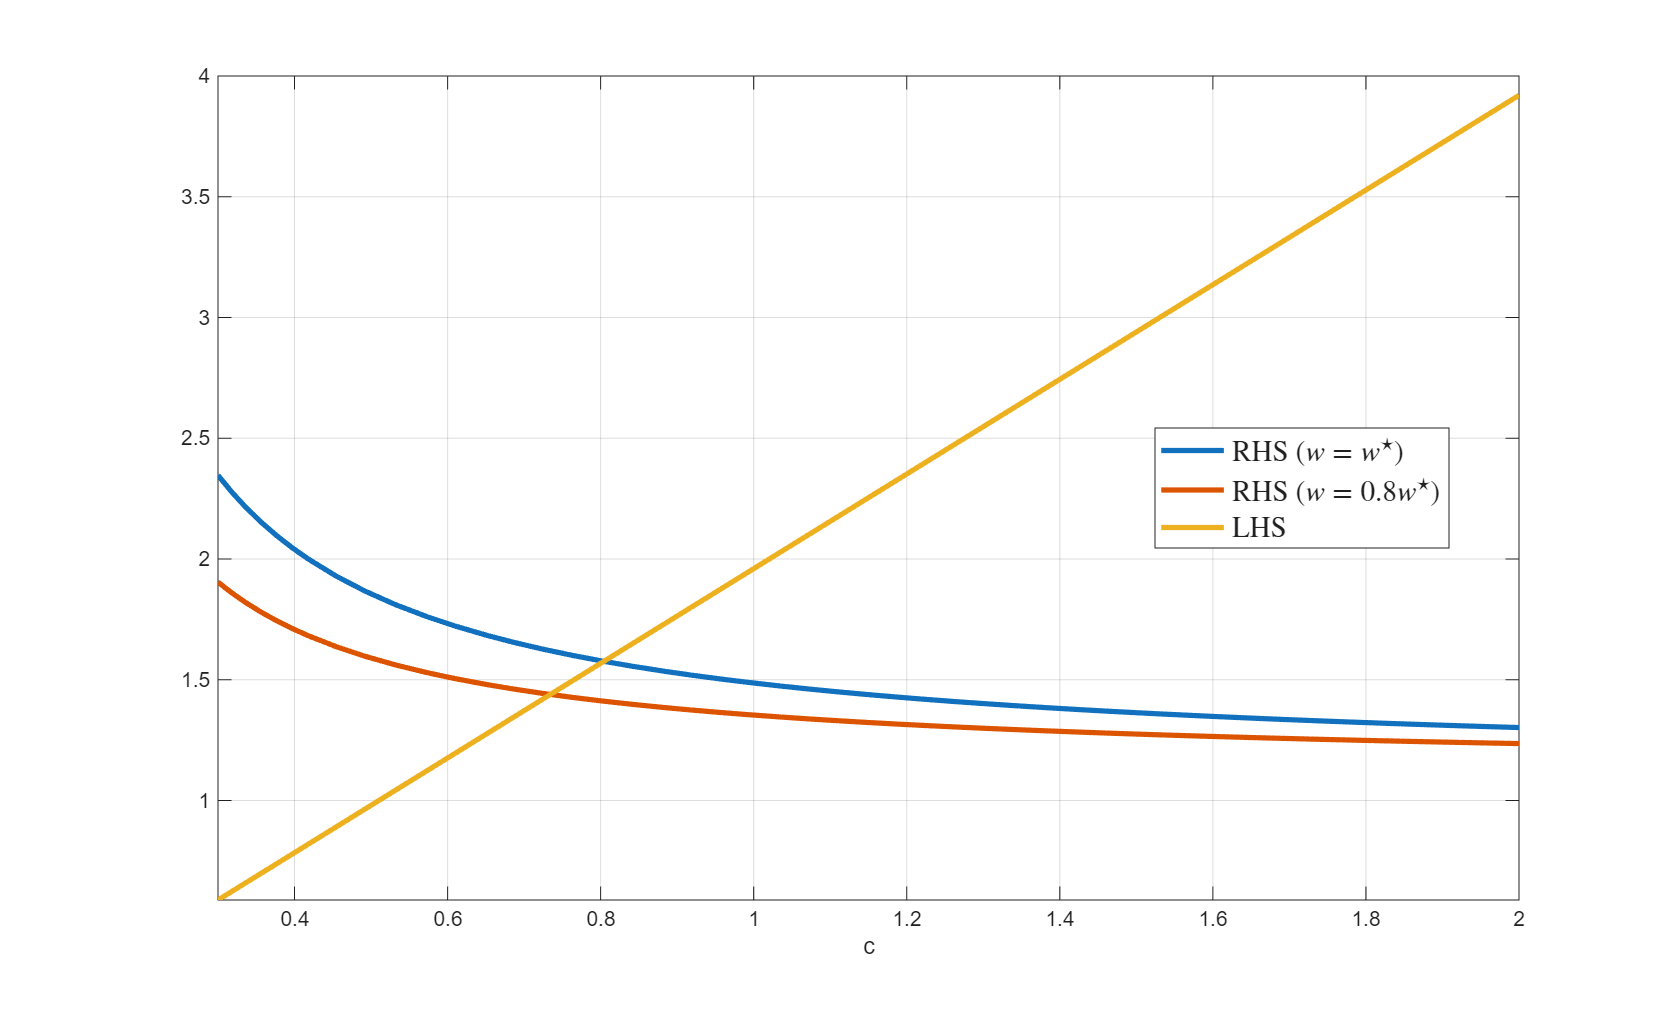
\includegraphics[width=\linewidth]{_figures/consumption_plot.png}
\end{subfigure}%
\begin{subfigure}{.5\textwidth}
  \centering
    \caption{Excess labour supply on the aggregate level.}
    \label{fig:a1_bisection}
  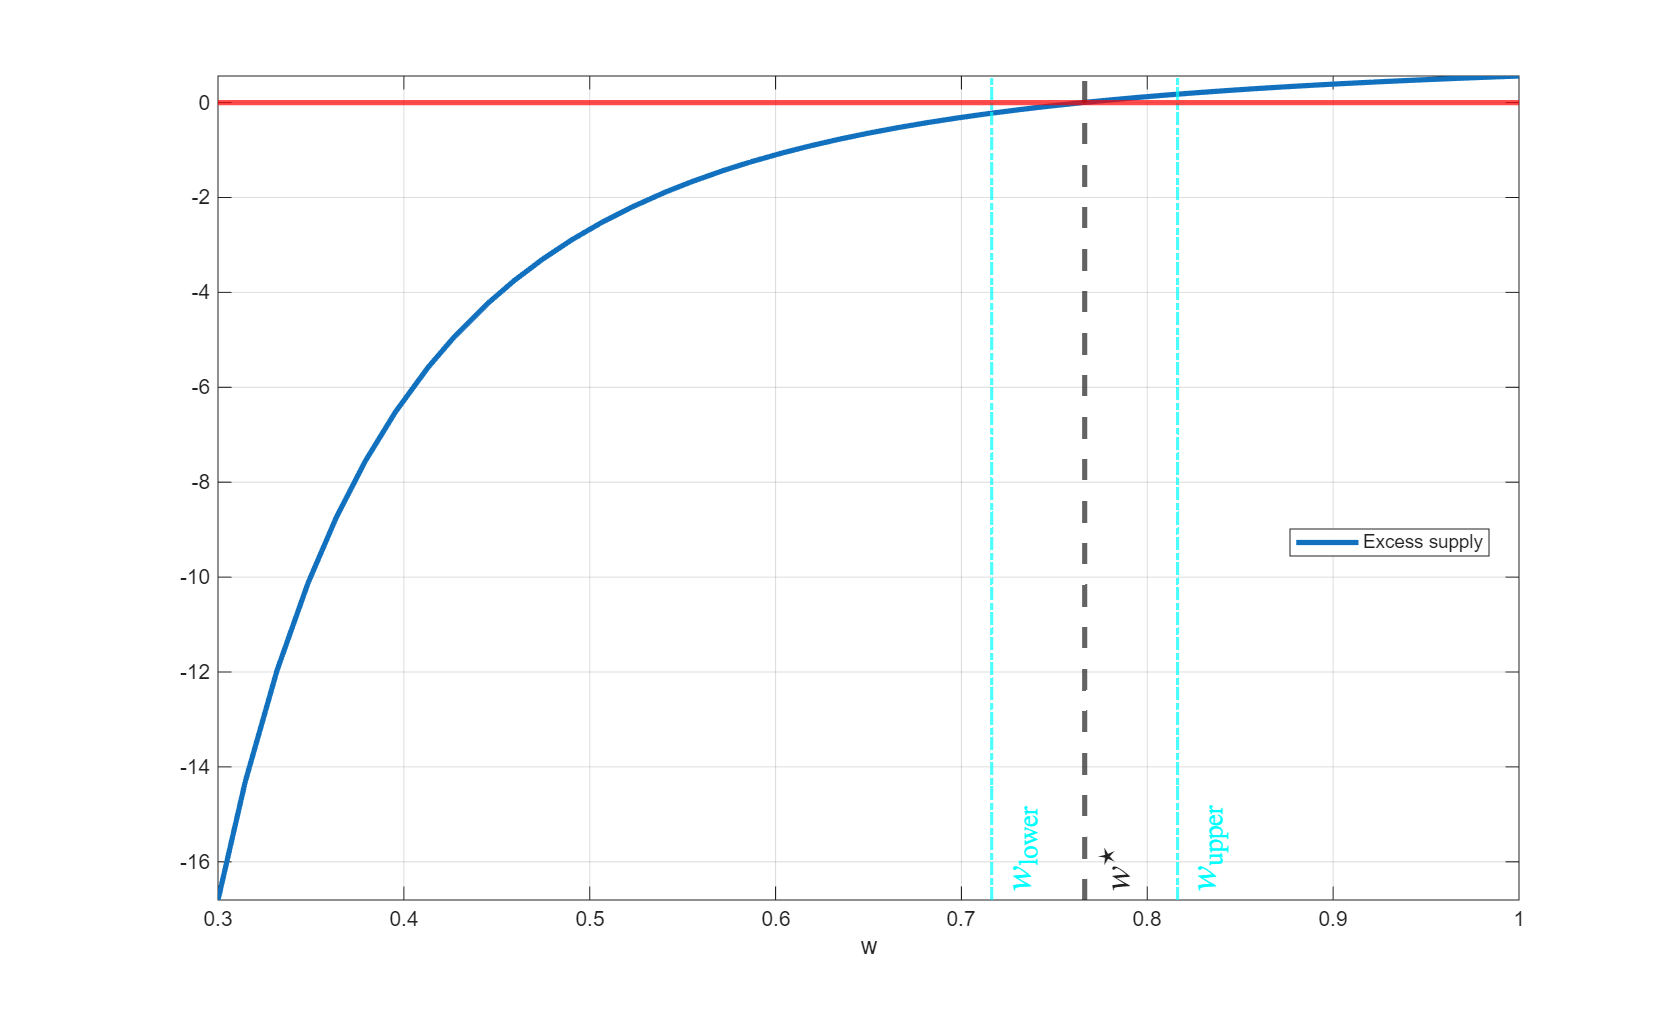
\includegraphics[width=\linewidth]{_figures/excess_supply_bisection.png}
\end{subfigure}
\end{figure}	
